\documentclass[a4paper,10pt]{article}
\usepackage[utf8]{inputenc}
\usepackage{graphicx}
%
%opening
\title{}
\author{}

\begin{document}

\maketitle

%\begin{abstract}

%\end{abstract}

\section{Automatic generation of neural mass model kernels}
\subsection{High level description of a simulation of a network of neural masses}
Neural mass models (NMMs) are mathematical tools to describe ensabled behaviour of groups of neurons through time. 
These models contain a set of internal states which describe the system and a set of coupled differential equations which define how the states of the system evolve.
An instance of these models is called a node.
The output of the model consists of a set of observables which identify states of interest for other nodes.
Nodes are linked to each other using a coupling function.
This coupling function is the equivalent of a synapse in a point neuron network.
Coupling defines how the input coming from other nodes should be treated.
Usually the coupling involves weighting the incoming signals by a factor and then passing this through a simple function.
The weights used for the coupling are of such level of detail that are matchable to connectivity maps which can be obtained from experimental measurements, e.g. tractography.

Certain observables of a neural mass can be post-processed to produce simulated BOLD, EEG and EMG signals among others. 
These signals can afterwards be input to an analysis step where a measure of the ability of the model to reproduce given aspects of the signal is performed.
The amount of open degrees of freedom in the Neural Mass Models generates a vast parameter space. 
The nature of the workflow described above allows the iterative modification and exploration of parameters in this admissible space.
Brute force of more intelligent approaches can be used to optimize the behaviour of the models with respect to fitness functions defined by experts and related to the essential characteristics of the higher level signals.

A general description of the simulation can be seen in Figure \ref{fig}
\begin{figure}
  \begin{center}
    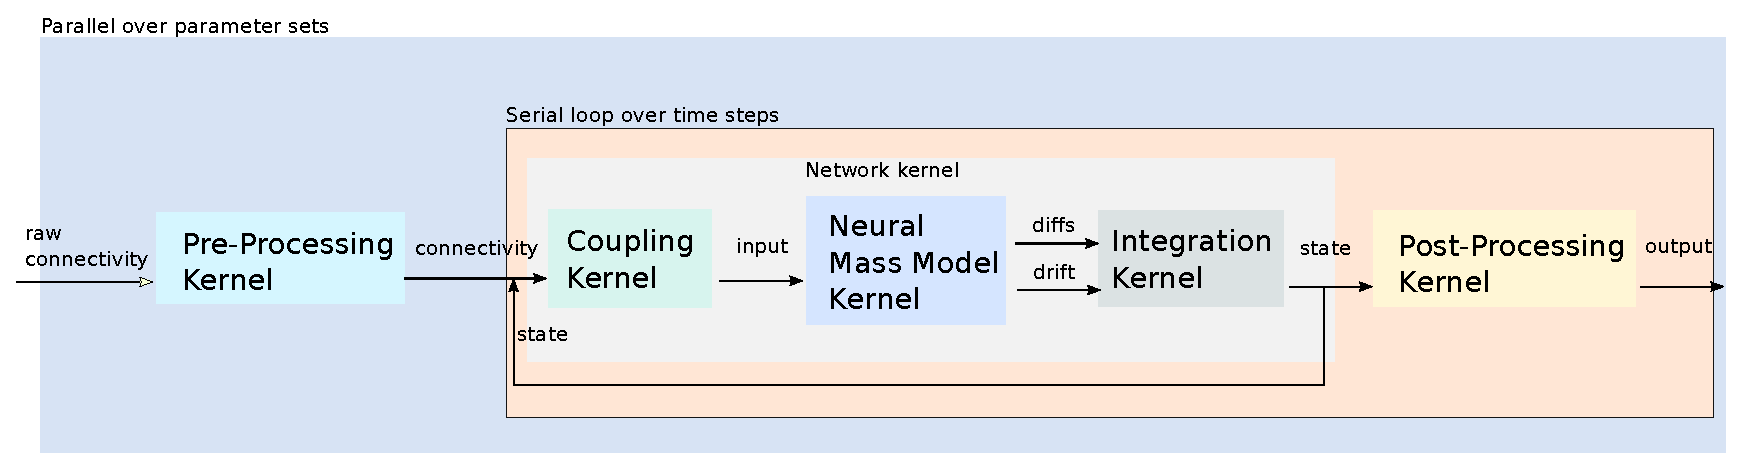
\includegraphics[scale=0.4]{DiagramNMM.eps}
  \end{center}
  \caption{Diagram of the interaction between the different computation stages in a neural mass model simulation.}
  \label{fig}
\end{figure}

\subsection{High level description of neural mass models}
In order to ease the high level description of the computation models used in this workflow, we have implemented the BaseModel class.
This class defines a set of attributes: 
\begin{enumerate}

\item State: Stores the internal states of the model.
\item Auxex: Auxiliary mathematical expressions which are used for internal calculations in the model.
\item Input: Stores the input comming from other neural masses into this neural mass.
\item Drift: Set of equations which transfer the model from a state at t-1 to another at time t.
\item Diffs: Differentiable variables in the system.
\item Observ: Observers are the data structures which contain inner states which must be available to the outside of the model. They represent the output of the model.
\item Const: Constant values specifically defined for a each model. 
\item Param: Parameters provided to an specific model. 
\item Limit: Defines the min and max limits within which the state values must be wrapped to ensure mathematical consistency.
 
\end{enumerate}


\subsection{Loopy as automatic code generation library}
Loopy \cite{loopy2014} is a python library intended to aid the automatic generation of parallel kernels for different target hardware platforms.
It includes targets for CUDA, OpenCL, KNL and CPUs.
Parallel code in Loopy is generated by enclosing a set of functions into an independent execution domains.
The dimensions of these domains are specified using inames. 
These inames represent the number of parallel instances that one can process at the same time of the given set of functions.

Other feature of loopy is the integration of multiple kernels into a single one.
The set of independent kernels is combined using a data flow which defines how variables are sent from one kernel into the next as input.
This allows the creation of complex kernels where data dependencies are assured.

Loopy automatically analizes the data structures used within the domain and the access patterns to them. 
The user can specify type and ranges for values and access limits to the data structures to control the way the data is handled.
Loopy assambles the computation within a loop-like environment, where each iteration is independent.
The code can then be specifically ported to a target platform using its specific language.

\subsection{Implementation of neural mass models with Loopy}
Our objective is to have a high level description of neural mass models which can then be used to automatically generate high performance parallel code for multiple platforms.
To achieve this goal with Loopy, we need to match the high level description language of the models to the specific API of Loopy.

The BaseModel class has functions which translate the information provided in the attributes of a model instance 
Generate the data structures
Define the kernel domain
Define the types for the attributes of the model
Generate expressions for constant deffinition
We unpack the values for the input, state and parameters.
Generate expressions for the auxiliary expressions
Generate expressions to store observables
We use pybolic to build a set of symbolic expressions representing the drift, diffs and observables.
We wrap the output within certain limits to avoid numerical inaccuracies. 

\bibliographystyle{abbrvnat}
\bibliography{references}

\end{document}
